\documentclass{article}
\usepackage[margin=.5in]{geometry}
\usepackage{graphicx, dblfloatfix}
\usepackage{amsmath, amssymb, amsfonts, mathrsfs, mathtools, physics}
\usepackage{gensymb}
\usepackage[english]{babel}
\usepackage[autostyle, english = american]{csquotes}
\usepackage[normalem]{ulem}
\usepackage[title,titletoc,toc]{appendix}
\usepackage{pgfplotstable}
\usepackage{array, booktabs, colortbl, caption}
\usepackage{braket}
\MakeOuterQuote{"}

\newcommand{\redchi}{$\tilde{\chi}^2\,$}
\renewcommand{\vec}[1]{\mathbf{#1}}

\title{Optical Absorption Edge in Semiconductors}
\author{Alejandro Legarda}

\begin{document}
\raggedright
\maketitle

\begin{abstract}
We investigate the transmittance and absorption of different semiconducting materials to determine the characteristics of their energy gaps. We determine whether the materials have a direct or indirect gap, and we measure the location of this gap, $E_g$. Our experimental data records transmittance, which we use to determine reflectance and refractive index, the former of which we use to determine and plot the absorption coefficient of each material against incident photon energy.
\end{abstract}
	
	
\tableofcontents
\newpage

\section{Theory}

\subsection{Energy Bands}

Atoms have discrete electron energy levels, but when atoms are brought together to form a solid, the electron orbitals overlap and interact to form wider energy bands. Such bands represent a continuum of allowed energies and adjacent bands may either overlap or be separated by a band gap depending on the structure and atoms that make up the material.\cite{lab manual}

\hspace{.25cm}


\begin{figure}[!htb]
	\centering
	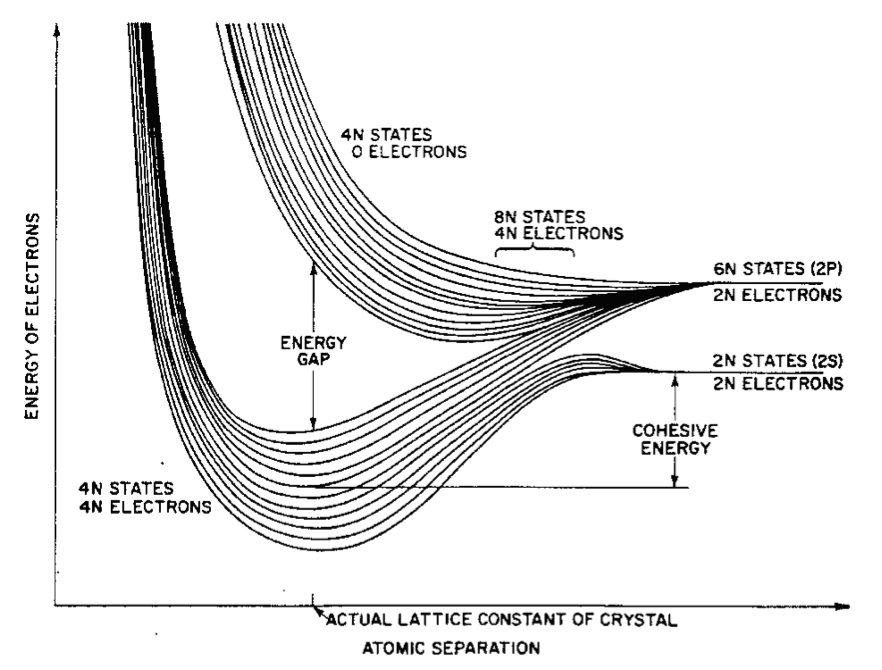
\includegraphics[scale=1.]{plots/fig_1.png}
 	\label{bands}
	\caption{An example of energy levels broadening into energy bands and energy gaps. N atoms, each with 4 electrons, move from distinct s and p energy states at large separation (far right of the plot) to two nearly continuous bands at smaller separation.\cite{lab manual}}
\end{figure}

\hspace{.25cm}

Electrons organize themselves within bands of a solid analogously to the discrete energy levels of a single atom. The innermost (core) electrons are bound tightly to the nuclei and fill the lowest energy bands. The valence electrons contribute to chemical bonds. The next higher energy band is the conduction band. Electrons in the conduction band are no longer bound to the nucleus and can thus move freely in the material. Electrons can be excited from the valence band into the conduction band by the absorption of energy from incident photons or from phonons. When an electron is excited from the valence to the conduction band, it leaves behind a hole of +1 charge in the valence band. An excited electron can return to the valence band by means of recombination with the hole.

\hspace{.25cm}

In semiconductors, the valence and conduction bands are separated by a small band gap, typically 0.1-1 eV. At room temperature, some electrons are thermally excited to the conduction band, but most remain in the valence band. The smallness of the band gap, however, means electrons can be promoted from the valence to conduction bands by absorption of photons with energies near the visible range. There are two factors that influence the size of the band gap. First, the gap widens when atoms connected by covalent bonds are smaller and hence can get closer together. Second, the gap widens as the bonds go from being more covalent to more ionic as it becomes easier to strip off electrons rather than share them.\cite{lab manual}

\hspace{.25cm}

\subsection{Momentum}

The momentum of electrons in a solid is also constrained in an analogous way. The DeBroglie relation $\vec{p} = \hbar \vec{k}$, where $\vec{k}$ is the wavevector that must satisfy the boundary conditions of the electron wavefunction in whatever medium (solid lattice) it is contained. The constraints on momentum depend on the physical properties of the lattice in question. There are so many levels within a band gap however, (on the order of $10^{23}$) that the energy spectrum can be considered continuous across values of k, as shown below.

\begin{figure}[!htb]
	\centering
	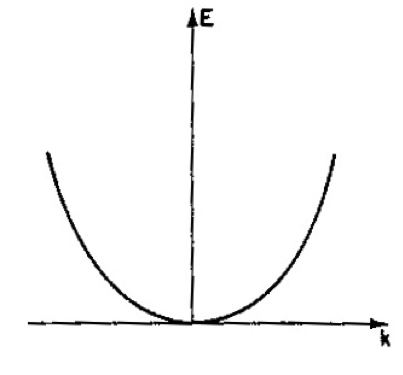
\includegraphics[scale=1.]{plots/fig_3.png}
 	\label{quadratic}
	\caption{Energy has a quadratic distribution with the wavevector $\vec{k}$.\cite{lab manual}}
\end{figure}

\subsection{Absorption}

In the visible region of the light spectrum, semiconductors are highly reflective  and highly absorptive ? typically having coefficients of absorption of the order of $\alpha \approx 105 cm^-1$.
The absorption coefficient is defined according to

\begin{equation}
	I_t = I_i \exp{-\alpha d}
\end{equation}

where $I_i$ is the incident intensity of the light and $I_t$ is the transmitted intensity after traveling a distance d through a material with absorption coefficient $\alpha$. The coefficient $\alpha$ depends on the photon energy. In semiconductors the absorption coefficient can vary radically with photon energy because of fundamentally different responses to photons with energies larger or smaller than the band gap energy.\cite{lab manual}

\hspace{.25cm}

With semiconductors, as incident photon energy decreases from visible toward the infrared, one will observe a sudden increase in transmission followed by a spectral region in which the semiconductor is more transparent. This fundamental absorption edge lies at a photon energy which is just sufficient to excite electrons across the energy gap $E_g$ which separates the valence band from the conduction band. The magnitude of the gap is an important factor determining the optical, electrical, and photoelectrical properties of the semiconductor.

In this experiment we determine the band gap energy for GaAs, Si, and Ge semiconductors from measurements of $\alpha(E)$ through the optical absorption edge. The transition from opaque to transparent is gradual and encodes considerable information.\cite{lab manual}

The rate at which a photon of a given energy is converted into an electronic excitation is given by Fermi?s Golden Rule: the rate is proportional to both the density of electrons available to absorb the photon and the density of available unoccupied final states, and to the sum of probabilities for transitions between these states. This implies that (a) if the energy of the photon is less than the gap energy, no electron-hole pairs can be created and the absorption rate is zero, and (b) as the energy rises above the band gap energy, the number of final states increases in a calculable way.\cite{lab manual}

Momentum must also be conserved for any transition, so the wavevector $\vec{k}$ must remain constant for the system (and in the case of the wavevector the quantity is dominated by the electron's contribution). We need only account for transitions where the sum of the wavevectors of the excited electron and hole add up to zero.\cite{lab manual}

Thermal excitations add another layer of information to the solid state. Because of room temperature at the start and during the experiment, the semiconductors do not start at ground state. To account for such excitations, one must average over the thermally excited initial states.\cite{lab manual}

\subsection{Direct versus indirect band gap}

Semiconductors fall into two categories based on the shape of their band structure.
\hspace{.25cm}
A direct band gap semiconductor is one where initial and final states of the electron have the same wavevector and no intermediate processes are required to conserve momentum when a photon is emitted or absorbed. (See Fig. 3.) The transition rate is governed only by the photon energy.\cite{lab manual}

\begin{figure}[!htb]
	\centering
	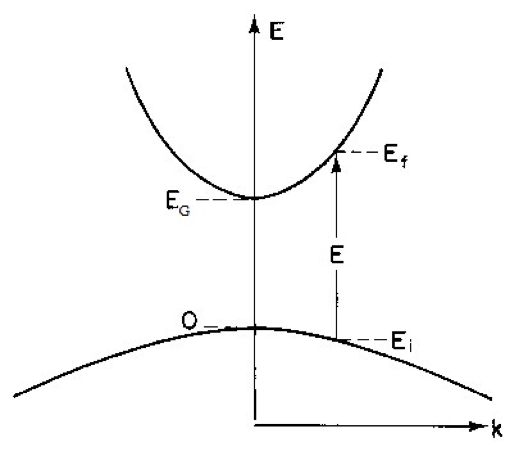
\includegraphics[scale=1.]{plots/fig_6.png}
 	\label{direct}
	\caption{Bands near a direct gap.\cite{lab manual}}
\end{figure}

According to Pankove (p. 36), the absorption coefficient is zero when $E < E_g$, but then grows when $E > E_g$ as

\begin{equation}
	\alpha(E) = A \sqrt{E - E_g},
\end{equation}
where A is a constant.

In an indirect band gap semiconductor the highest occupied electronic state not only has a different energy than the lowest empty energy state, but a different wavevector as well. (See Fig. 4.) Optical transitions from the valence to the conduction band can therefore occur only when both a photon and a phonon are involved. The phonon must have a wavevector equal to the difference in wavevector of the two bands.

\begin{figure}[!htb]
	\centering
	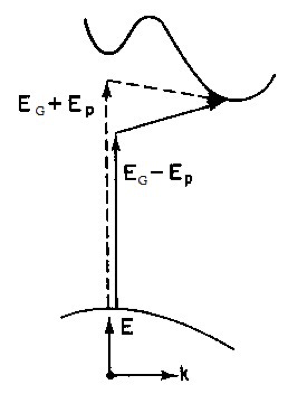
\includegraphics[scale=1.]{plots/fig_7.png}
 	\label{indirect}
	\caption{Bands near an indirect gap.\cite{lab manual}}
\end{figure}

If the phonon has energy $E_p$, then the absorption coefficient for a transition with phonon absorption at photon energy $E > E_g - E_p$ is

\begin{equation}
	\alpha_a(E) = B(E - (E_g - E_p))^2,
\end{equation}

where B is a constant, and the absorption coefficient for a transition with phonon emission at photon energy $E > E_g + E_p$ is

\begin{equation}
	\alpha_e(E) = C(E - (E_g + E_p))^2,
\end{equation}

where C is a constant. It is worth noting that when the photon has energy $E > E_p + E_g$, both absorption and emission are possible, and $\alpha(E) = \alpha_a(E) + \alpha_e(E)$.


\section{Experimental Method}
\subsection{Apparatus}

We use a Beckman spectrophotometer to measure the fraction of light intensity as a function of wavelength transmitted through different semiconductor samples. This instrument uses a chopping technique to make alternating measurements of the intensity of the light with and without a sample in the optical path. The ratio of the two intensities is used to determine the fractional transmission, or transmittance, T of the sample,

\begin{equation}
	T = \frac{I_t}{I_i},
\end{equation}
where $I_i$ is the intensity of the light in the absence of the sample and $I_t$ is the intensity after passing through the sample, as before.

\begin{figure}[!htb]
	\centering
	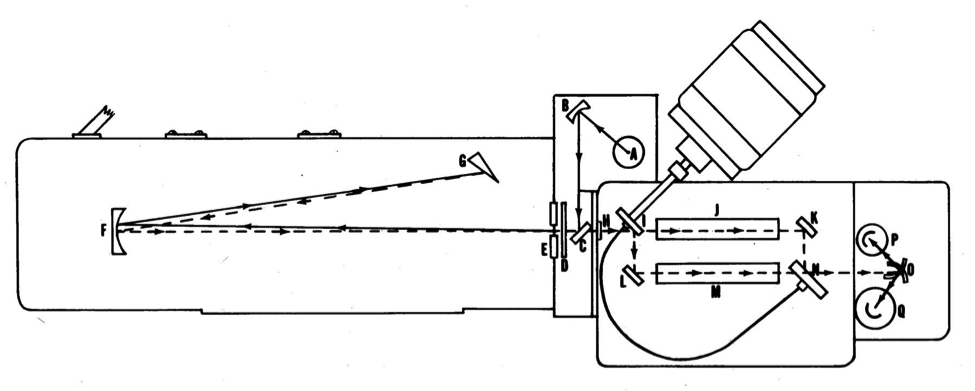
\includegraphics[scale=1.]{plots/fig_8.png}
 	\label{beckman}
	\caption{Optical path for Beckman Spectrophotometer.\cite{lab manual}}
\end{figure}

A schematic of the instrument is shown in Fig. 5. "Light from the source (A) is focused on the slit (E) by the condensing mirror (B). The directed beam from the condensing mirror (B) is deflected through the chopper (D) and upon the entrance slit (E) by the slit entrance mirror (C). Light focused on the slit (E) falls on the collimating mirror (F) and is rendered parallel and reflected to the quartz prism (G). The back surface of the prism is aluminized so that light is reflected back through the prism. The desired wavelength of light is selected by rotating the wavelength selector which adjusts the angular position of the prism. The spectrum is directed back to the collimating mirror (F) which focuses the selected wavelength in the slit (E). Light leaving the monochronometer is focused by the lens (H) into the sample compartment, where the beam is alternately switched between the reference path (J) and the sample path (M) by rotating mirrors (I and N) and stationary mirrors (L and K). The beam entering the photocell compartment is focused by the spherical condensing mirror (O) on either the lead sulfide detector (P) or the photomultliplier detector (Q)."\cite{lab manual}

\hspace{.25cm}

In order to compensate for changes in measured intensity of the signal in the Reference channel, due to the spectral shape of the blackbody spectrum for example, the spectrophotometer uses a feedback circuit to control the width of the slit (E) so as to maintain constant intensity of the Reference signal. The ratio of the Sample signal to the Reference signal gives the fractional transmission of the sample.\cite{lab manual}

\subsection{Calibration}

We calibrate our apparatus in order to maximize the use of its dynamic range. We follow the procedure detailed:
\hspace{.25cm}
\begin{itemize}
\item With no samples in the sample chamber, lid is placed on the chamber.
\item Wavelength is set to ~1000 nm.
\item Open both the Sample and Reference shutters. The pen holder on the X-Y plotter moves up to near the $100\%$ mark.
\item $100\%$ dial is adjusted so that the pen holder points to the $100\%$ mark.
\item Now Sample shutter is closed, and the pen holder falls to near the $0\%$ mark.
\item Zero dial is adjusted so that the pen holder points to $0\%$.
\end{itemize}

\hspace{.25cm}

We used a voltmeter and knowledge of the apparatus' dynamical range to quantify the response to $0\%$ and $100\%$ voltage levels and calibrate the apparatus (see Table 1). We took a second set of calibration data at the end of the second day, for more robust calibration through averaging to account for drifts (see Table 2).

\begin{table}[]
\centering
\caption{Calibration data taken at the start of experiment}
\label{cal1}
\begin{tabular}{@{}llll@{}}
\toprule
Transmission \% & nm   & mV     & d(mV) \\ \midrule
0          & 2500 & 0.72   & 0.02  \\
0          & 2250 & 0.71   & 0.02  \\
0          & 2000 & 0.72   & 0.02  \\
0          & 1500 & 0.72   & 0.03  \\
0          & 1000 & 0.71   & 0.02  \\
0          & 650  & 0.72   & 0.02  \\
100        & 2500 & 24.07  & 0.1   \\
100        & 2250 & 24.37 & 0.07 \\
100        & 2000 & 24.35  & 0.06  \\
100        & 1500 & 24.75 & 0.07 \\
100        & 1000 & 24.47  & 0.06  \\
100        & 650  & 24.48 & 0.06 \\ \bottomrule
\end{tabular}
\end{table}

\begin{table}[]
\centering
\caption{Calibration data taken at the end of the experiment.}
\label{cal2}
\begin{tabular}{@{}llll@{}}
\toprule
Transmission \%  & nm   & mV     & d(mV) \\ \midrule
100 & 2500 & 24.02  & 0.03  \\
100 & 2250 & 24.69  & 0.03  \\
100 & 2000 & 24.69 & 0.07 \\
100 & 1500 & 24.79 & 0.07 \\
100 & 1000 & 24.41 & 0.06 \\
100 & 600  & 24.34 & 0.09 \\
0   & 2500 & 0.62   & 0.01  \\
0   & 2250 & 0.62  & 0.04 \\
0   & 2000 & 0.61  & 0.03 \\
0   & 1500 & 0.61  & 0.03 \\
0   & 1000 & 0.60  & 0.02 \\
0   & 600  & 0.60  & 0.03 \\ \bottomrule
\end{tabular}
\end{table}

\subsection{Data Collection}

For each semiconductor we scan across wavelengths to find the absorption edge of the material. We concentrate our data points around this transition region, recording transmittance against wavelength. Repeated measurements of the same points give us an estimate of random uncertainty.


\section{Analysis}
\subsection{Transmittance}

Using our calibration data, we determine $V_0$ and $V_{100}$, the 0 and $100\%$ transmittance voltages for the purpose of converting voltage signal, $V$, to transmittance,

\begin{equation}
	T = \frac{V - V_{100}}{V_{100} - V_0}.
\end{equation}

We will also convert wavelength to energy, using

\begin{equation}
	E = \frac{hc}{\lambda}.
\end{equation}

\begin{table}[]
\centering
\caption{Calibration results.}
\label{voltages}
\begin{tabular}{@{}lll@{}}
Transmittance \% & Voltage (mV) \\ \midrule
0                & 0.66 $\pm$ 0.02 \\
100              & 24.4  $\pm$ 0.06
\end{tabular}
\end{table}
 
We then plot the transmittance percentage against energy in order to make an estimate of the energy gap. See Table 4 for these estimates, which were taken visually and have a considerable uncertainty to account for this and the fact that we are most likely underestimating.

\begin{table}[]
\centering
\caption{Energy gap estimates for different semiconducting materials.}
\label{gap estimates}
\begin{tabular}{@{}ll@{}}
Material & Energy Gap Estimate ($10^{-19}$J) \\ \midrule
Si       & 1.70 $\pm$ 0.05                            \\
Ge       & 1.05 $\pm$ 0.05                          \\
GaAs     & 2.15 $\pm$ 0.05                         
\end{tabular}
\end{table}

\begin{figure}[!htb]
	\centering
	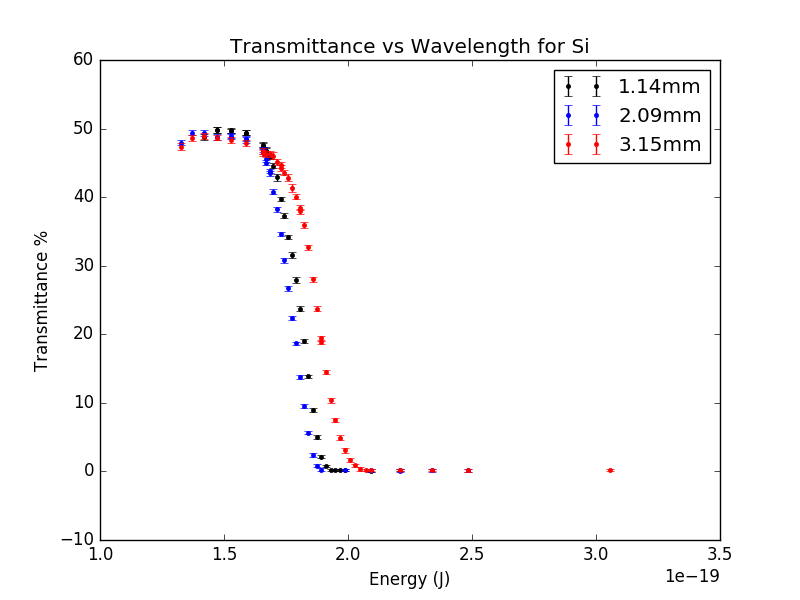
\includegraphics[scale=.75]{plots/Si.png}
 	\label{Si}
	\caption{Data for all three thicknesses of silicon.}
\end{figure}

\begin{figure}[!htb]
	\centering
	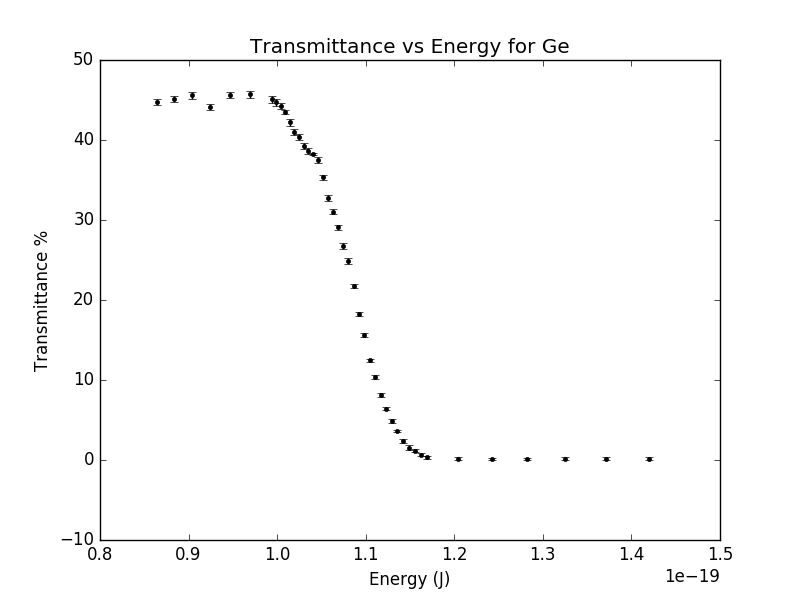
\includegraphics[scale=.75]{plots/Ge.png}
 	\label{Ge}
\end{figure}

\begin{figure}[!htb]
	\centering
	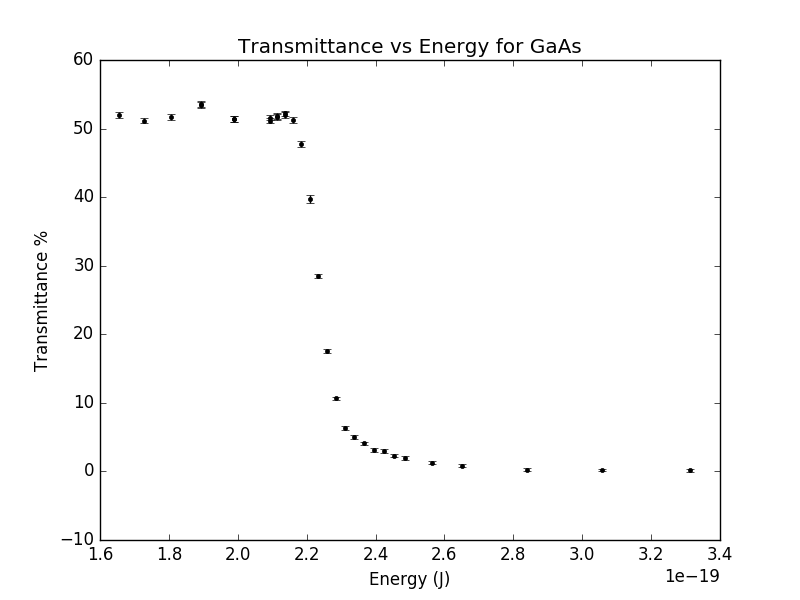
\includegraphics[scale=.75]{plots/GaAs.png}
 	\label{GaAs}
\end{figure}

\begin{table}[]
\centering
\caption{Maximum transmittance factors}
\label{maxtran}
\begin{tabular}{@{}ll@{}}
Material & $T_{\alpha=0}$  \\ \midrule
Si -  1.14mm      & 0.50 $\pm$ 0.01 \\
Si - 2.09mm       & 0.49 $\pm$ 0.01 \\
Si - 3.15mm       & 0.48 $\pm$ 0.01 \\
Ge       & 0.46 $\pm$ 0.01 \\
GaAs     & 0.53 $\pm$ 0.01
\end{tabular}
\end{table}

\subsection{Reflectance}

\begin{table}[]
\centering
\caption{}
\label{my-label}
\begin{tabular}{@{}llll@{}}
\toprule
Material    & $T_{\alpha=0}$  & Reflectance, R  & Refractive index, n \\ \midrule
Si - 1.14mm & 0.50 $\pm$ 0.01 & 0.33 $\pm$ 0.01 & 5.8 $\pm$ 0.2       \\
Si - 2.09mm & 0.49 $\pm$ 0.01 & 0.34 $\pm$ 0.01 & 5.7 $\pm$ 0.2       \\
Si - 3.15mm & 0.48 $\pm$ 0.01 & 0.35 $\pm$ 0.01 & 5.5 $\pm$ 0.2       \\
Ge          & 0.46 $\pm$ 0.01 & 0.37 $\pm$ 0.01 & 5.2 $\pm$ 0.2       \\
GaAs        & 0.53 $\pm$ 0.01 & 0.31 $\pm$ 0.01 & 6.4 $\pm$ 0.2       \\ \bottomrule
\end{tabular}
\end{table}

Knowing the reflectance coefficients for the semiconductors, we can calculate their refractive indexes using the relation in equation (8)

\begin{equation}
	R = [\frac{n-1}{n+1}]^2.
\end{equation}

\subsection{Absorption}

We then use our data to calculate the absorption coefficient,

\begin{equation}
	\alpha = \frac{1}{d} ln[\frac{(1-R)^2 + \sqrt{(1-R)^4 + 4T^2 R^2}}{2T}].
\end{equation}

\begin{figure}[!htb]
	\centering
	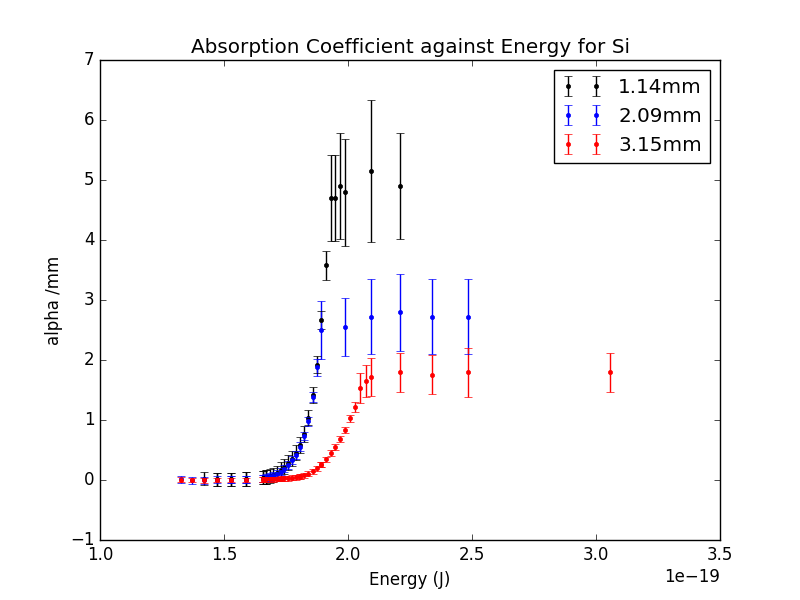
\includegraphics[scale=.75]{plots/Si_alpha.png}
 	\label{Si_a}
	\caption{Data for all three thicknesses of silicon.}
\end{figure}

\begin{figure}[!htb]
	\centering
	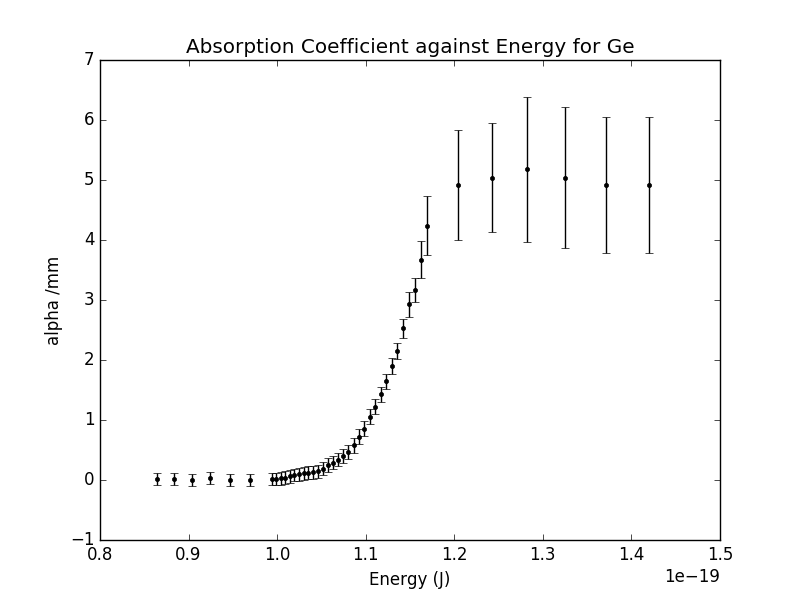
\includegraphics[scale=.75]{plots/Ge_alpha.png}
 	\label{Ge_a}
\end{figure}

\begin{figure}[!htb]
	\centering
	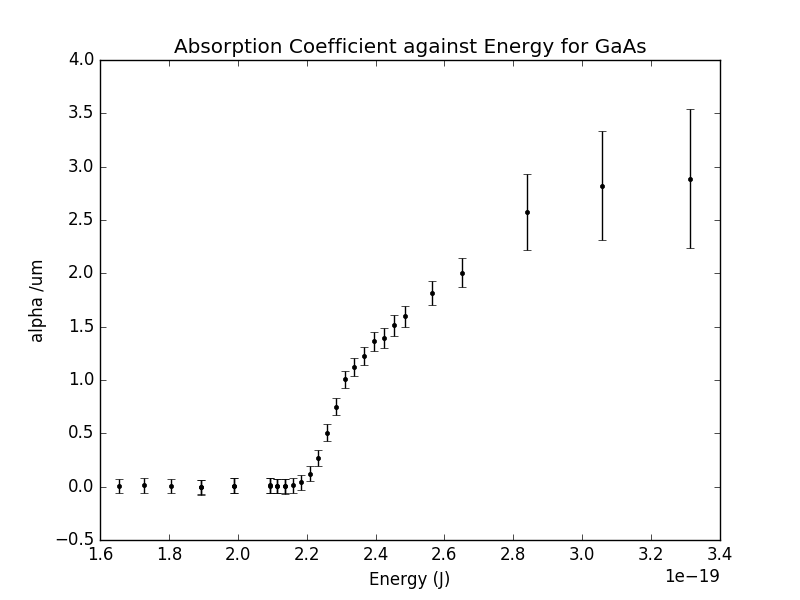
\includegraphics[scale=.75]{plots/GaAs_alpha.png}
 	\label{GaAs_a}
\end{figure}

Based on the absorption against energy plot, and looking at the functional forms of equations (3) and (4), we can determine that Silicone and Germanium have indirect band gaps, whereas Gallium Arsenide has a direct band gap. This is apparent in the steeper slopes for Si and Ge. The absorption coefficients for the three different silicon thicknesses converge near low energies as expected. Identifying GaAs as a direct band gap semiconductor, we can plot $\alpha^2$ against energy and fit the linear region in order to determine the energy gap, $E_g$.

\begin{figure}[!htb]
	\centering
	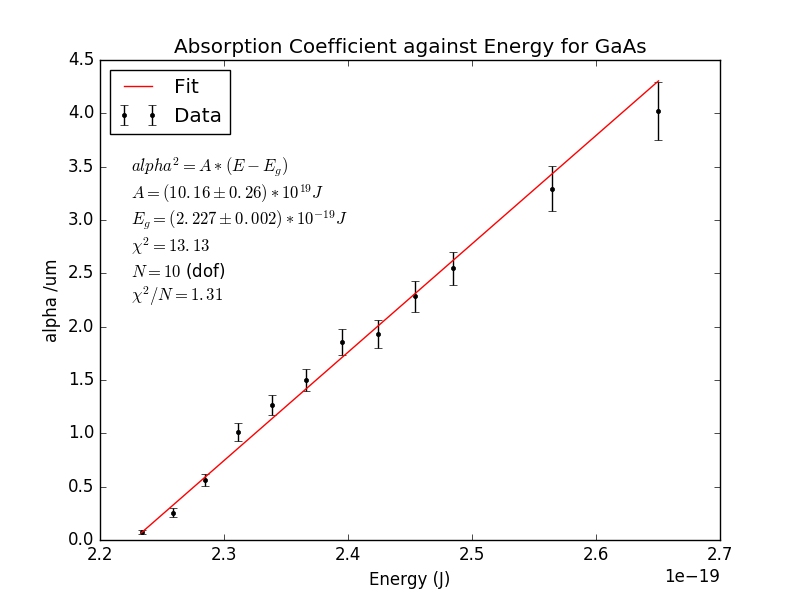
\includegraphics[scale=.75]{plots/GaAs_alpha_fit.png}
 	\label{GaAs_a}
	\caption{We extract $E_g$ from the x-intercept of this fit. As we can see, it agrees within $2\sigma$ of our rough estimate from earlier. It seems likely from this plot that we underreported uncertainties.}
\end{figure}

\subsection{Error Analysis}

Here we will show the full treatment from error, $\Delta V$ in a raw data point, $V$, to the final error in $\alpha$ for a single datum. We found that fractional uncertainties were appropriate for propagation in the simple relationships for T and R. Proper error propagation is then used for the more complicated formula for $\alpha$.

\begin{gather}
	\Delta T =  [\frac{\Delta V}{V} + 2*\frac{\Delta V_0}{V_0} + \frac{\Delta V_{100}}{V_{100}}] * T \\
	\Delta E = \frac{\Delta V}{V} * E
\end{gather}

Let us take the data point $V =  11.99 \pm 0.04mV, wavelength = 910nm$, and use the values for $V_0 and V_{100}$ (and their uncertainties) from before. We then calculate

\begin{gather}
	T = 0.285 \\
	\Delta T =  [\frac{0.04}{11.99} + 2\frac{\Delta V_0}{V_0} + \frac{\Delta V_{100}}{V_{100}}] * 0.285 \\
	\Delta T = 0.003 \\
	E = 2.23e-19 \\
	\Delta E = \frac{0.04}{11.99} * 2.23e-19
\end{gather}

We used points $T_{\alpha=0}$ to find the reflectance coefficient, so for $\Delta R$

\begin{equation}
	\Delta R = 2 * \frac{\Delta T_{\alpha=0}}{T_{\alpha=0}} * R.
\end{equation}


\section{Conclusion}

Our energy band gap values all fall within $2\sigma$ of the accepted literature values (Table 7).

\begin{table}[]
\centering
\caption{Results comparison against literature.}
\label{my-label}
\begin{tabular}{@{}lllll@{}}
\toprule
Material & \multicolumn{2}{l}{$E_g$ (eV)}  & \multicolumn{2}{l}{Refractive index, n} \\ \midrule
         & Experimental Value & Literature \cite{gaps} & Experimental Value     & Literature  \cite{refractive}   \\
Si       & $1.06 \pm 0.03$    & 1.11       & $5.5 \pm 0.2$          & 3.42           \\
Ge       & $0.67 \pm 0.03$    & 0.66       & $5.2 \pm 0.2$          & 4.06           \\
GaAs     & $1.34 \pm 0.03$    & 1.43       & $6.4 \pm 0.2$          & 3.29           \\ \bottomrule
\end{tabular}
\end{table}


\begin{thebibliography}{10}

	\bibitem{lab manual}
		University of Chicago Department of Physics. "Optical Absorption Edge in Semiconductors"\\
		https://wiki.uchicago.edu/display/P211manuals/Optical+Absorption+Edge+in+Semiconductors. (Accessed May, 2016)

	\bibitem{taylor}
		Taylor, John. \emph{An Introduction to Error Analysis}. Sausalito: University Science Books, 1997.
		
	\bibitem{refractive}
		Refractive Index Database\\
		http://refractiveindex.info/. (Accessed May, 2016)
		
	\bibitem{gaps}
		Kittel, C., \emph{Introduction to Solid State Physics}, 6th Ed., New York: John Wiley, 1986, p. 185.
		
\end{thebibliography}

\end{document}